\subsection{Implementación de Overdrive en MATLAB}

%comentar que script se utiliza

Se implementa en MATLAB un overdrive simple dado por la siguiente expresón:
\begin{align}
    x' &= G_i x \\ 
    y' &= \begin{cases}
    \beta x' + \text{sign}(x')(1-\beta) \alpha \hspace{2 cm} &\text{si }\abs{x'} \geq \alpha\\
    x' &\text{si }\abs{x'} < \alpha
    \end{cases}\\
    y &= G_o y'
\end{align}

La función implementada se muestra a continuación:

\lstinputlisting[language = octave]{Code/overdrive.m}

Posteriormente se aplica dicha función al archivo de audio \texttt{gtr\_jazz.wav} obteniendo el audio \texttt{gtr-ov\_a02b005Gi1Go1.wav} el cual utiliza $\alpha = 0.2, \beta = 0.05$ y $G_i = G_o = 1$. Se adjunta el audio resultante a la entrega. 
\\
Con respecto a la percepción auditiva, se pecibe una clara distorsión en el sonido. Lo anterior se le atribuye a que la función overdrive es no lineal por lo tanto cambia el contenido en frecuencias de la señal.
\\
\newline
Se pide aplicar el efecto a una señal de audio adecuada para una comparación visual de lo que hace el efecto sobre la señal. Se considera \texttt{gtr\_jazz.wav} un buen audio para lo anterior, pues debido a sus claros cambios de intensidad en el sonido se pasa de zona lineal a no lineal con frecuencia.

En la figura \ref{fig:p211} se muestra el audio \textit{gtr-.wav} original y luego de aplicar overdrive. Se nota claramente que la distorsión cumple su cometido, añadiendo cambios bruscos en la señal, lo cual puede interpretarse como que se agregaron componentes de alta frecuencia.

\begin{figure}[H]
    \centering
    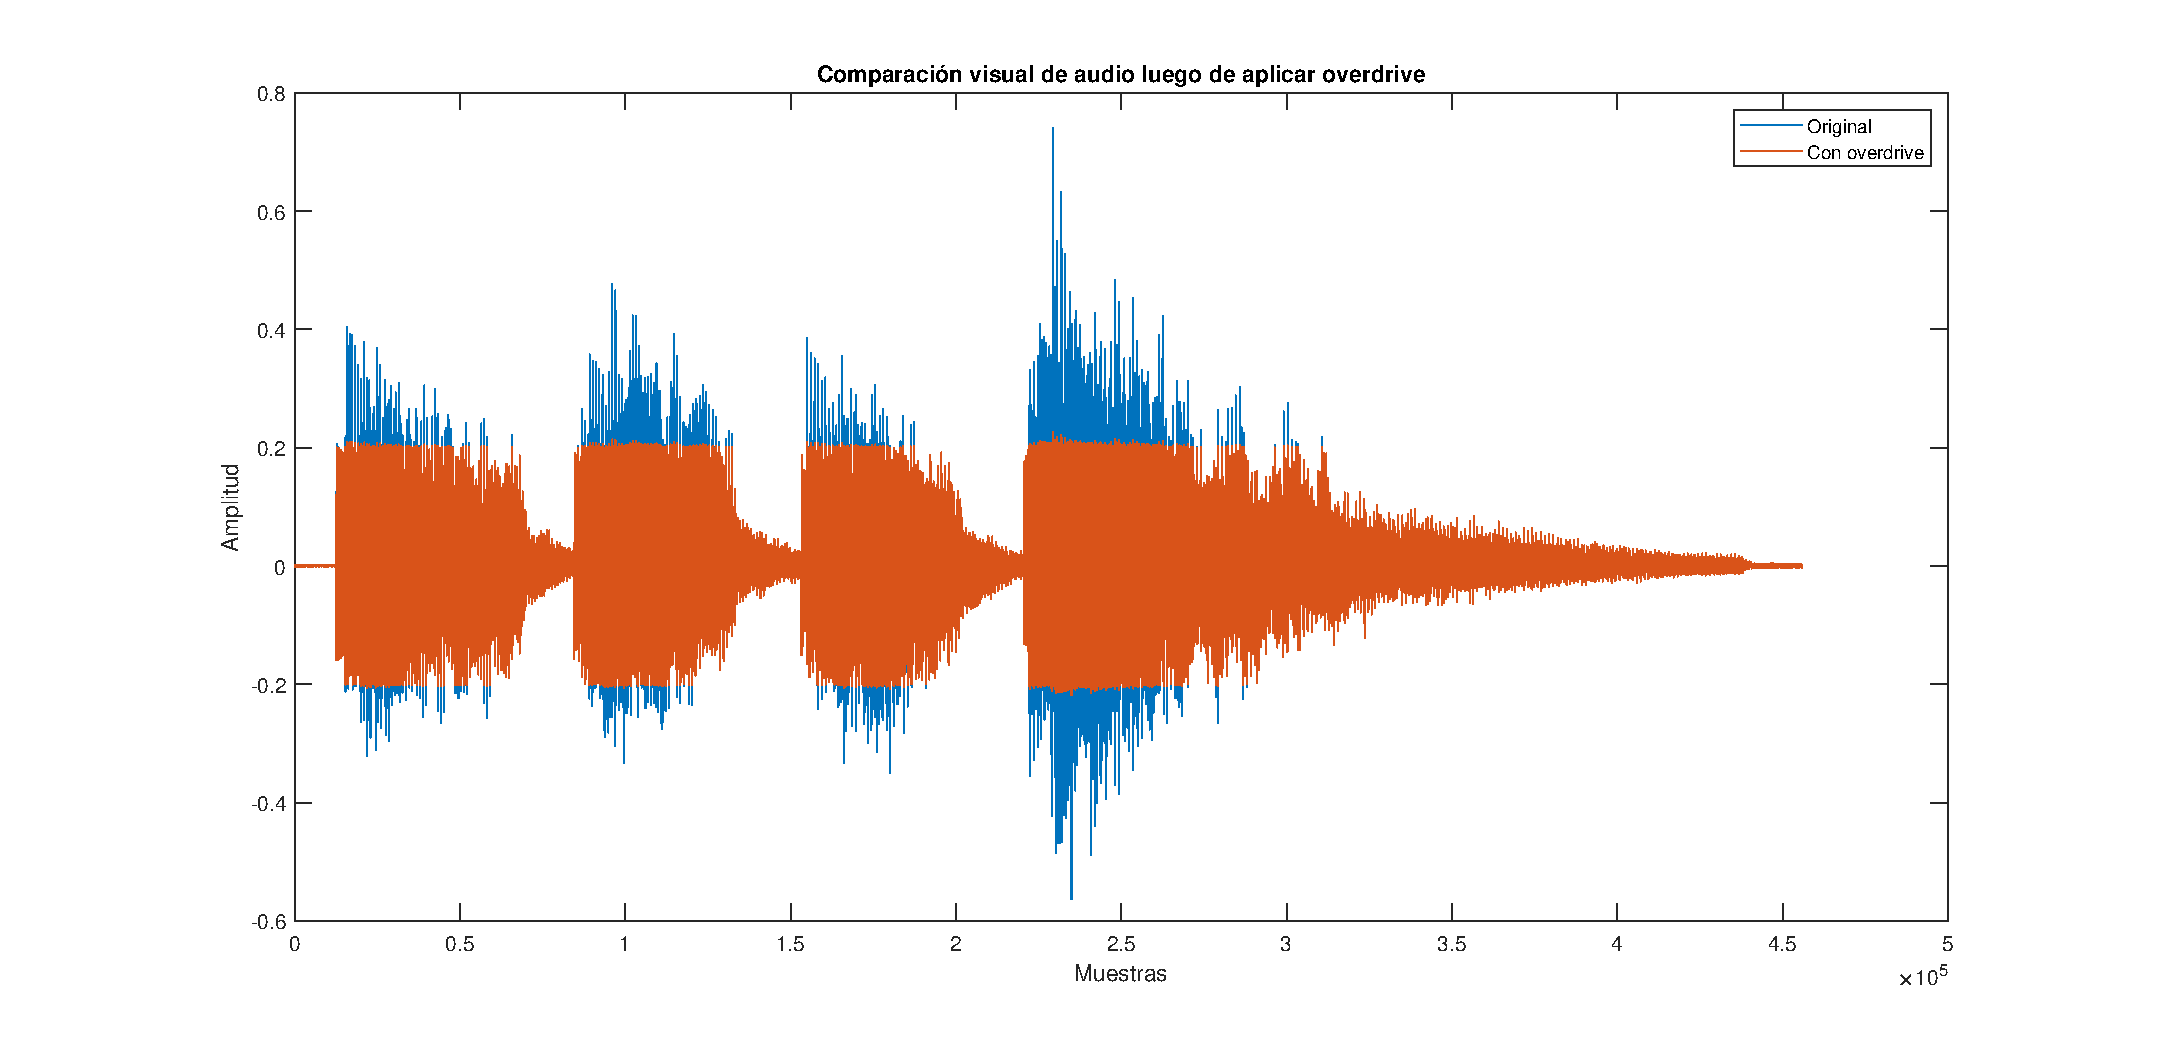
\includegraphics[width = .8\linewidth]{Figuras/p211_comparacion-overdrive.eps}
    \caption{Audio \textit{gtr-.wav} original y luego de aplicar overdrive.}
    \label{fig:p211}
\end{figure}

Posteriormente se analiza que ocurre al variar los parámetros de la función, tomando $\alpha=0.1$ y $G_i = 3$. La relación salida/entra de este overdrive y el original se muestra en la figura \ref{fig:p212}.

\begin{figure}[H]
    \centering
    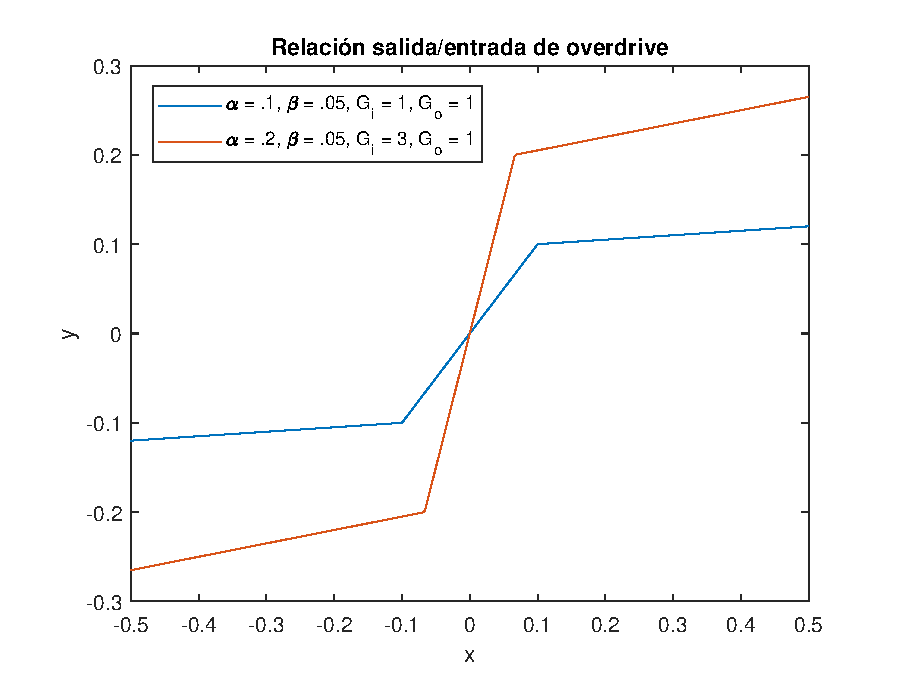
\includegraphics[width = .8\linewidth]{Figuras/p212_relacion-overdrive.eps}
    \caption{Relación Salida/Entrada de overdrive con distintos parámetros.}
    \label{fig:p212}
\end{figure}

A partir de la figura \ref{fig:p212} se aprecia que el overdrive con los nuevos parámetros genera una señal con menos energía que el anterior, pues cada punto azul es menor en magnitud a su punto rojo correspondiente para algún valor $x$ de entrada. Lo anterior podría corregirse variando $G_o$. Por otro lado vemos que con la nueva combinación de parámetros el cambio de pendiente es aparentemente menos abrupto, por lo que se esperaría una percepción auditiva menor en el overdrive. Además, la zona lineal aumenta, lo cual es otra razón para que la percepción auditiva de la distorsión producto al overdrive sea menor.

Los parámetros del modelo de overdrive utilizado pueden interpretarse de la siguiente forma:
\begin{itemize}
    \item $G_i$: Ganancia de entrada. la cual sirve para balancear que la señal $x'$ ''se mueva'' por los intervalos de no linealidad. Si $G_i$ es muy bajo no habrá distorsión. 
    \item $\alpha$: Umbral de no linealidad. Si $\alpha$ es muy alto no hay distorsión pues $x$ estaría en zona lineal. De la misma forma si $\alpha$ es muy pequeño no se aprecia distorsión.
    \item $\beta$: Relacionado a que tan abrupto es el cambio de pendiente en el módulo no lineal (ecuación de $y'$). Afecta a la percepción de la distorsión. 
    \item: $G_o$: Ganancia de salida. Está relacionada con el ''volumen'' de la señal de salida. No genera distorsión.
\end{itemize}

\subsection{Implementación de un Delay Multi-Tap}

Una implementación de un delay multitap corresponde a la siguiente expresión
\begin{equation}
    y[n] = \sum_{k=1}^N b(k)x[n-k\cdot M]
\end{equation}

Donde:
\begin{itemize}
    \item $x$: Señal de entrada
    \item $N$: Número de etapas de retardo.
    \item $M$: Número de muestras equivalentes a la longitud de cada retardo. Dado $T$ un retardo por etapa deseado en s y una $T_s$ periodo de muestreo, $M$ puede obtenerse como:
    $$M = \dfrac{T}{T_s}$$
    \item $b(k)$: Ganancia de la $k$-ésima etapa.
\end{itemize}

En primer lugar se solicita aplicar un delay multi-tap de 4 etapas ($N$) de longitud 125 ms ($T$) y ganancia constante $b(k) = 0.35$ al archivo \textit{gtr-jazz.wav}. 

Auditivamente se nota que el efecto de repetición de la señal a modo de ''eco'', sin embargo, el hecho de que $b(k)$ se mantenga constante hace que el sonido sea antinatural. El archivo de audio obtenido corresponde a \textit{gtr-jazz\_delay-multitap.wav}, el cual se adjunta en la entrega

La función creada para implementar el delay multi-tap en MATLAB se muestra a continuación:

\lstinputlisting[language = octave]{Code/delay_multitap.m}

Se decide que \textit{gtr-jazz.wav} es una buena señal para mostrar el efecto del delay muli-tap debido a los claros ecos escuchados en la señal de audio resultante. El gráfico resultante se muestra en la figura \ref{fig:p221}. 

\begin{figure}[H]
    \centering
    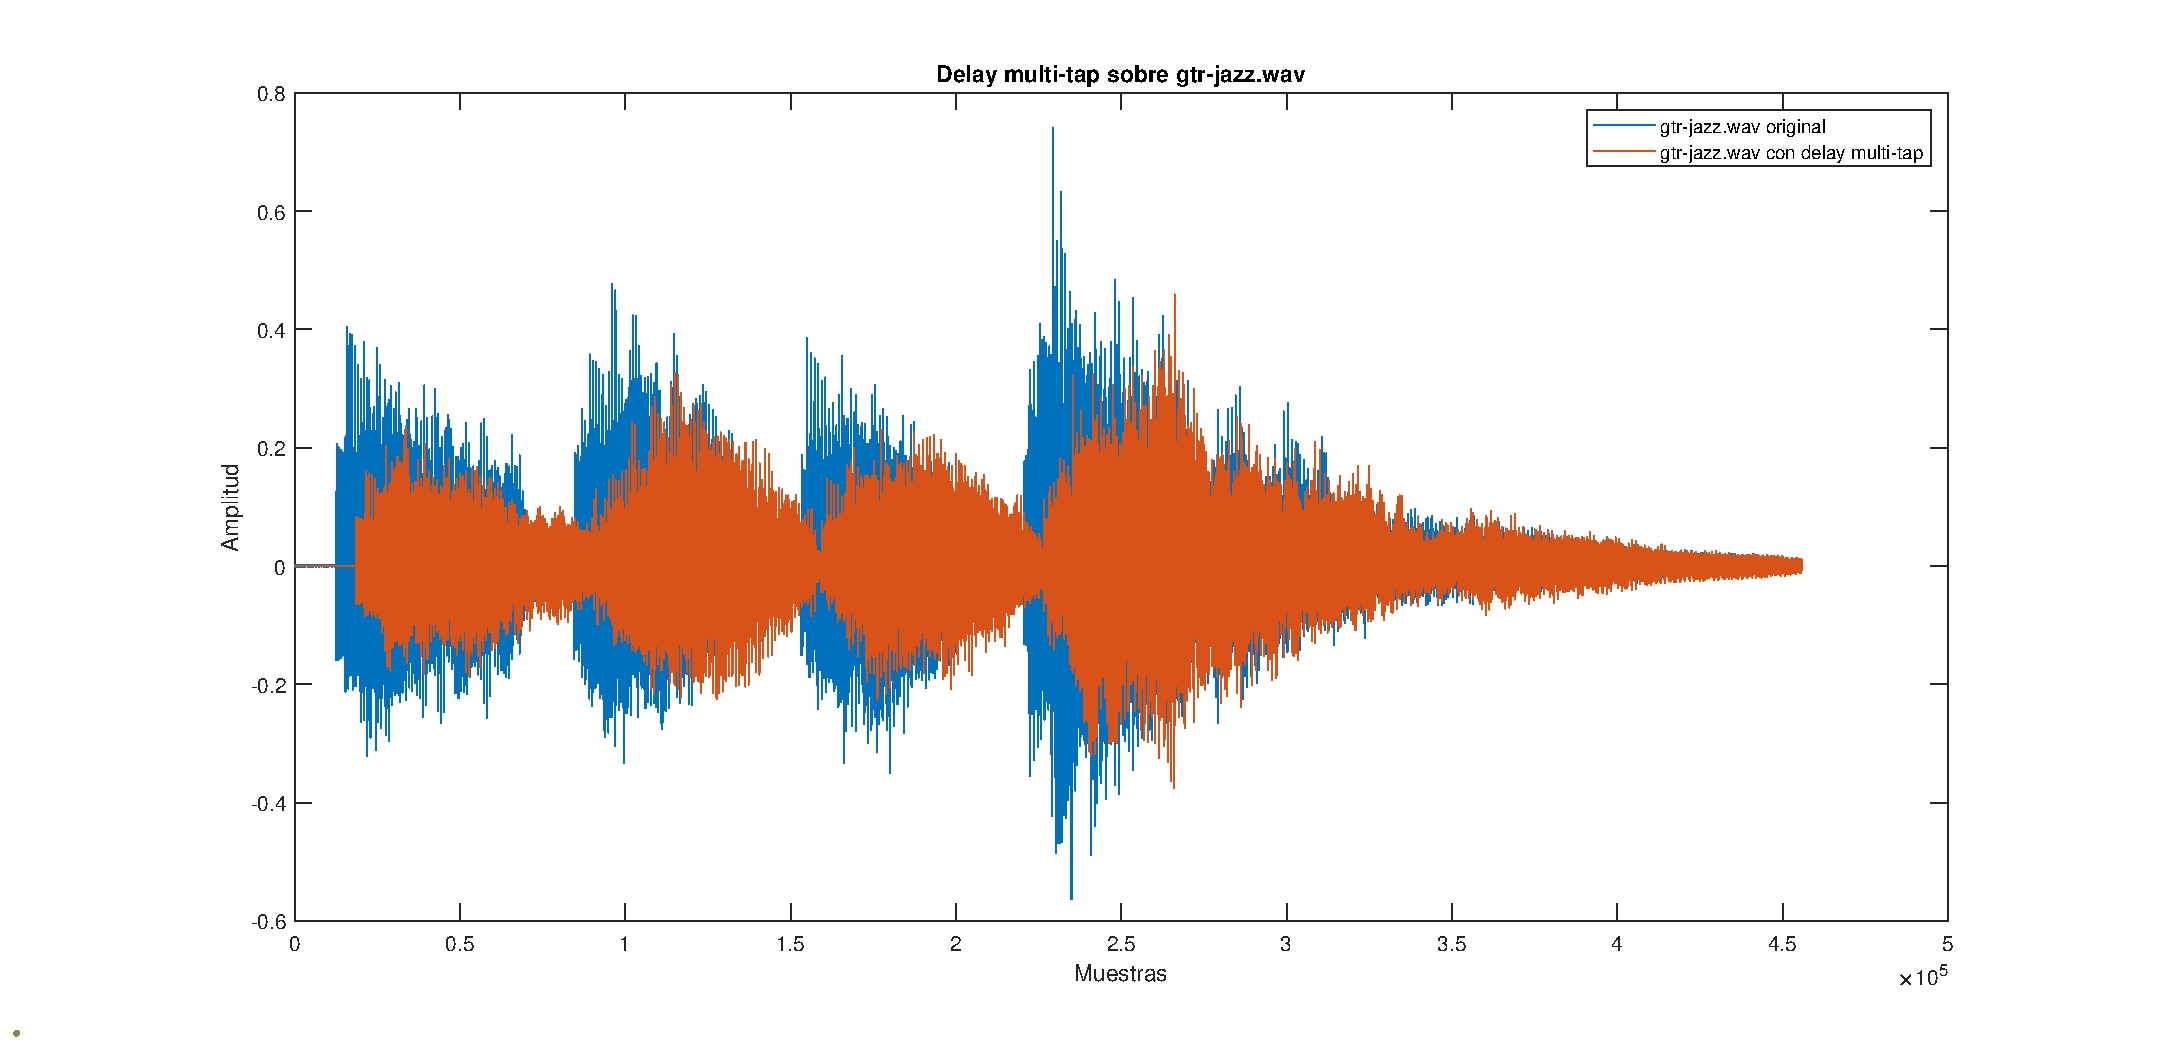
\includegraphics[width = .8\linewidth]{Figuras/p221_comparacion-delay.eps}
    \caption{Audio \textit{gtr-jazz.wav} original y luego de aplicar delay multi-tap.}
    \label{fig:p221}
\end{figure}

Curiosamente no se logra apreciar el eco de forma visual, pero si el efecto de filtro pasabajos que tiene un filtro de media móvil de ganancias constantes. Lo anterior se le atribuye a que el tiempo de retardo es muy bajo para la duración de los ''segmentos'' de la señal (arpegios).

Posteriormente se cambia $N=10$, $T = 250$ ms y $b(k) = 0.35^k$ y se vuelve a aplicar el efecto a \textit{gtr-jazz.wav}, obteniendo \textit{gtr-jazz\_delay-multitap2.wav}, el cual se adjunta en la entrega. Auditivamente se siente un decaimiento mucho más natural del eco. Una comparación gráfica se muestra en la figura \ref{fig:p222} , siendo notoria una mayor atenuación en la señal que con ganancias constantes.

\begin{figure}[H]
    \centering
    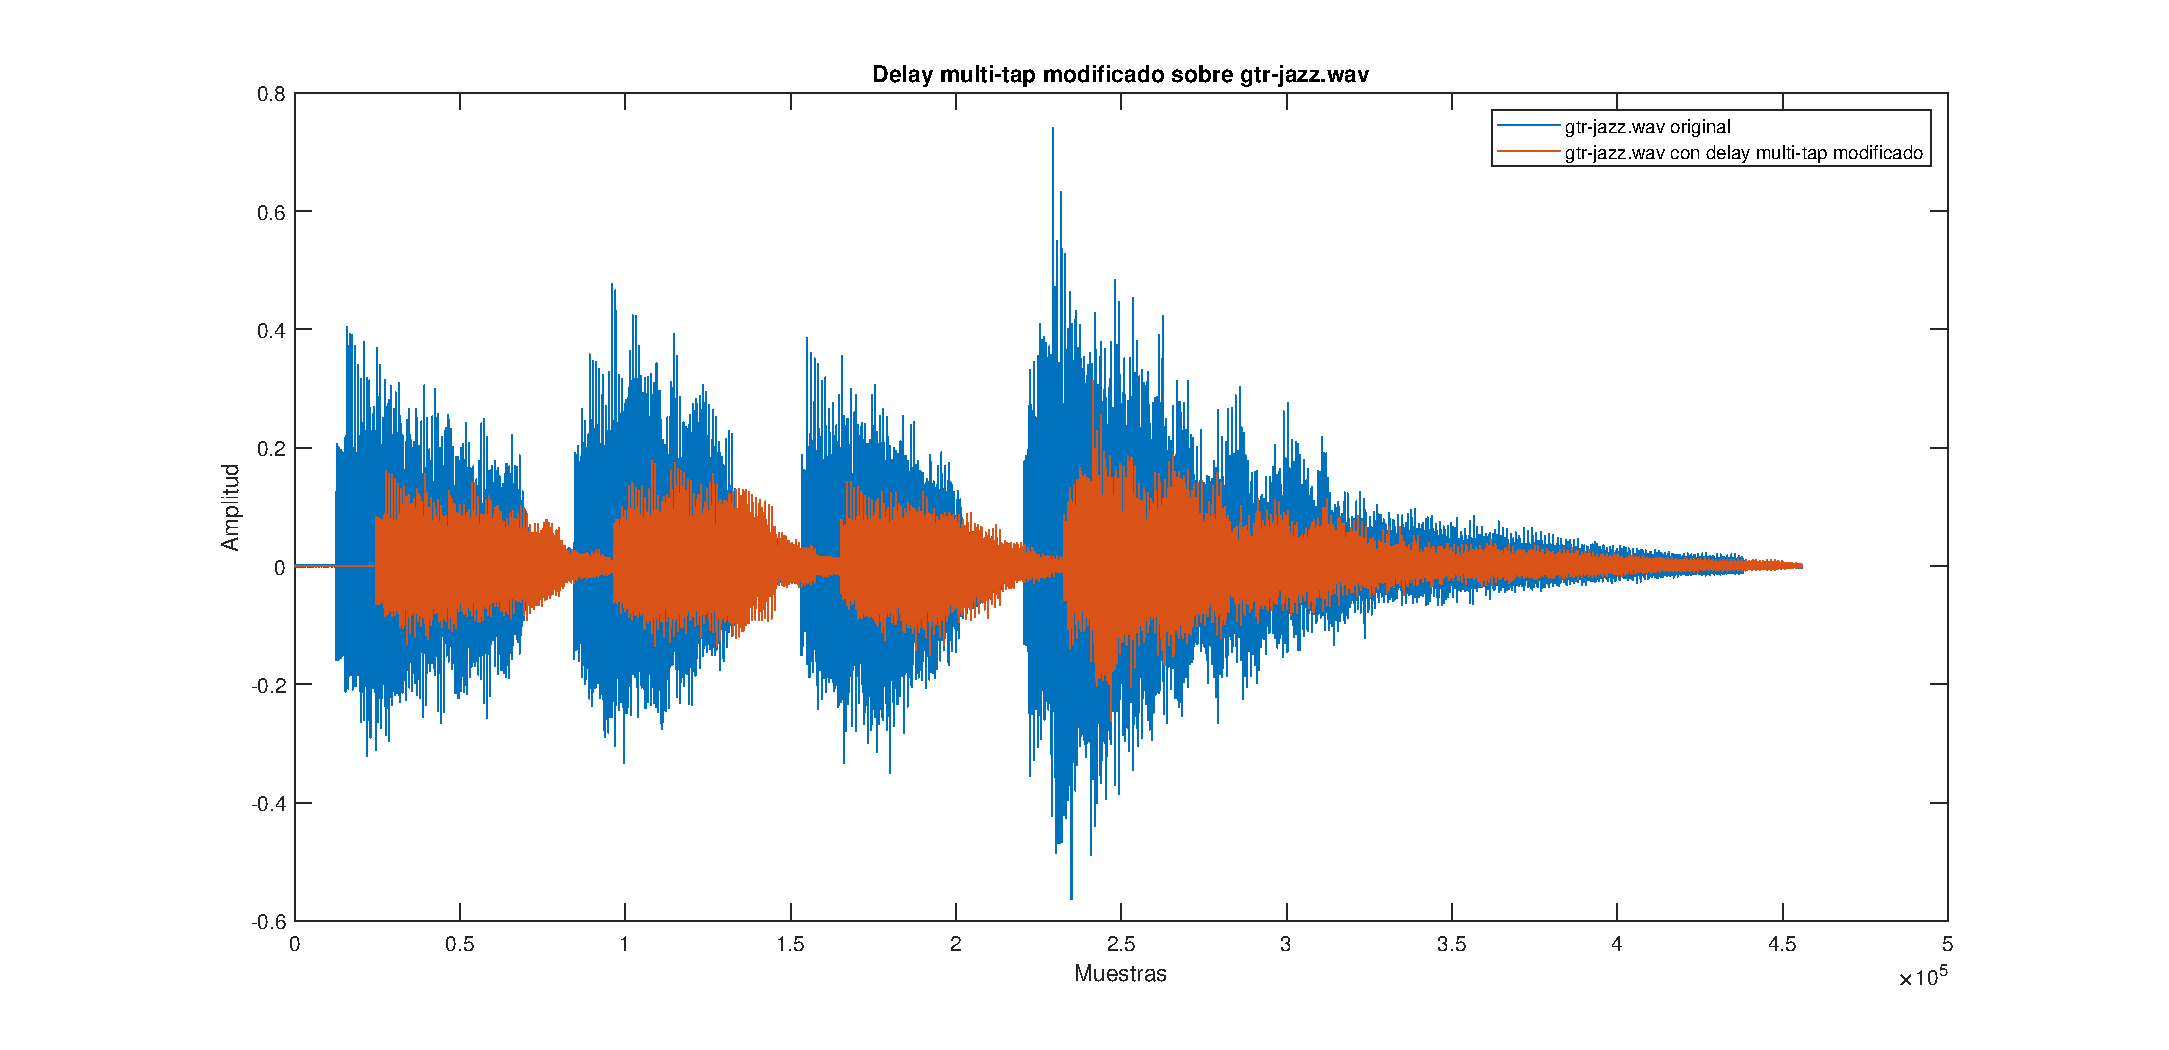
\includegraphics[width = .8\linewidth]{Figuras/p222_comparacion-delay.eps}
    \caption{Comparación entre audio \textit{gtr-jazz.wav} original y luego de aplicar delay multi-tap con ganancia $b(k) = 0.35^k$.}
    \label{fig:p222}
\end{figure}

Finalmente se modificó la frecuencia de muestreo en el audio \textit{gtr-jazz.wav} a 16 kHz usando el comando \texttt{resample}. El audio a la nueva frecuencia de muestreo se guardo en el archivo \textit{gtr-jazz\_resample-16.wav} el cual se adjunta con la entrega. Auditivamente no se escucha mayor diferencia con el audio original. Los parámetros elegidos para lograr el mismo efecto anterior corresponden a:
\begin{itemize}
    \item $N$: Se mantiene en 10, pues las etapas no cambian.
    \item $M$: Al cambiar la frecuencia de muestreo este cambia. Como la frecuencia de muestro original (48 kHz), es el triple de la nueva (16 kHz), ahora M corresponde a un tercio de las muestras anteriores.
    \item $b(k)$: Se mantiene pues no se cambia la ganancia por etapa.
\end{itemize}

El audio obtenido al aplicar los nuevos parámetros de delay sobre la señal a la nueva tasa de muestre se guarda en el archivo \textit{gtr-jazz\_resample-16\_delay.wav}, el cual se adjunta en la entrega. No se perciben diferencias auditivas notorias con el audio a 48 kHz.

Con respecto a las ventajas y desventajas de aplicar resample se tiene:
\begin{itemize}
    \item Ventajas: Menor tiempo de cálculo de la salida del filtro. En aplicaciones que tengan algún requisito de tiempo máximo para procesamiento puede ser útil.
    
    \item Desventajas: El cambio de frecuencia de muestreo puede provocar perdida de contenido espectral de interés.
\end{itemize}


